\documentclass[conference]{IEEEtran}

% ---------- Packages ----------
\usepackage{newtxtext,newtxmath} % Times系
\usepackage{amsmath}
\usepackage{siunitx}
\usepackage{graphicx,xcolor}
\usepackage{booktabs}
\usepackage{placeins}
\usepackage[hidelinks]{hyperref}

\usepackage{tikz}
\usetikzlibrary{calc,positioning,fit,arrows.meta,shapes.geometric,shapes.misc}

% ---------- TikZ styles ----------
\tikzset{
  line/.style={-Latex, line width=0.5pt},
  box/.style={draw, rounded corners, align=center, inner sep=3pt, font=\small},
  smallbox/.style={box, minimum width=25mm, minimum height=7mm},
  midbox/.style={box, minimum width=32mm, minimum height=9mm},
  bigbox/.style={box, minimum width=68mm, minimum height=10mm}
}

% ---------- Title ----------
\title{AITL on Space: A Robust Three-Layer Architecture with a Tri-NVM Hierarchy for Long-Duration Spacecraft Autonomy}

\author{
\IEEEauthorblockN{Shinichi Samizo}
\IEEEauthorblockA{Independent Semiconductor Researcher\\
Former Engineer at Seiko Epson Corporation\\
Email: shin3t72@gmail.com\quad GitHub: \url{https://github.com/Samizo-AITL}}
}

\begin{document}
\maketitle

% ---------- Abstract ----------
\begin{abstract}
We propose \emph{AITL on Space}, a robust three-layer architecture (Robust Core, FSM Supervisor, AI Adaptor) integrated with a tri-NVM hierarchy (SRAM, MRAM, FRAM) and mapped to a 22\,nm FD\!SOI SoC. The novelty lies in a complete flow from mission-level specification to ASIC implementation: requirements are formalized as JSON via EduController, synthesized by the AITL-H module, verified in FPGA HIL with fault injection, stress-tested through SystemDK FEM (thermal/radiation/packaging), and finally mapped to ASIC. This end-to-end methodology enables resilient autonomy for long-duration spacecraft missions.
\end{abstract}

% ============================================================
\section{Introduction}
Deep-space missions require ultra-robust control under total ionizing dose (TID), single-event effects (SEE), and thermal cycling. Conventional PID\,+\,Flash architectures face limits due to drift, aging, and endurance. We present AITL on Space: a three-layer control architecture with a hardened memory hierarchy, supported by a reproducible design flow from JSON specification to ASIC.

% ============================================================
\section{Specification and Design Flow}
The design process begins with mission requirements captured in EduController, exported as JSON including plant matrices and weighting functions. AITL-H consumes this JSON to synthesize an $H_\infty$ controller $K$ in fixed-point form. The resulting design undergoes FPGA HIL validation, followed by FEM co-simulation in SystemDK, before 22FDX ASIC tape-out.

% ---------- Fig.1 Design Flow ----------
\begin{figure}[t]
\centering
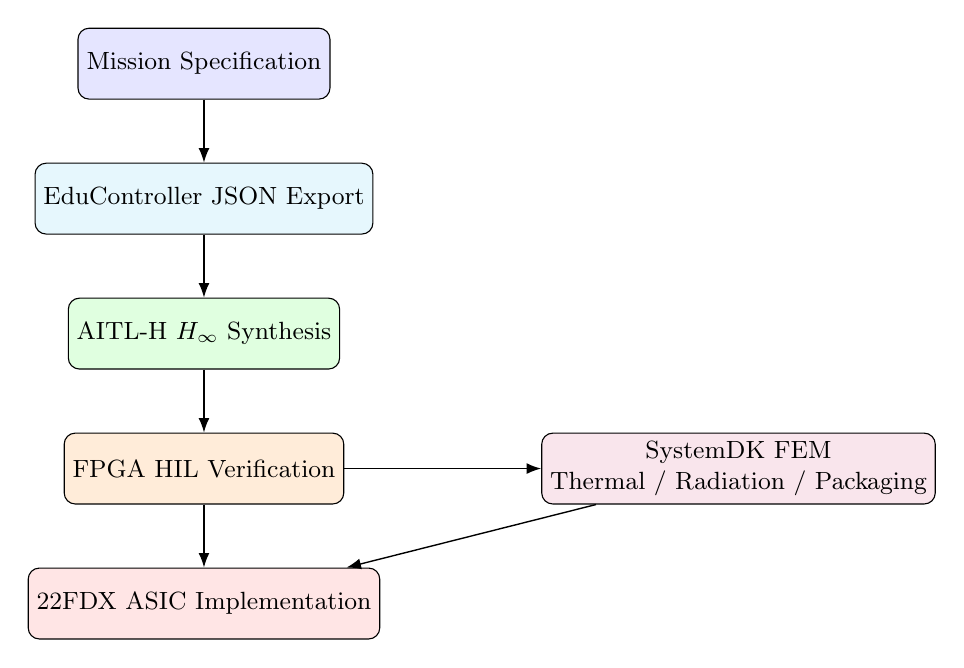
\begin{tikzpicture}[node distance=8mm]
  \node[midbox, fill=blue!10] (spec) {Mission Specification};
  \node[midbox, fill=cyan!10, below=of spec] (json) {EduController JSON Export};
  \node[midbox, fill=green!12, below=of json] (hinf) {AITL-H $H_\infty$ Synthesis};
  \node[midbox, fill=orange!15, below=of hinf] (hil) {FPGA HIL Verification};
  \node[midbox, fill=red!10, below=of hil] (asic) {22FDX ASIC Implementation};
  \node[midbox, fill=purple!10, right=25mm of hil] (fem) {SystemDK FEM\\Thermal / Radiation / Packaging};

  \draw[line] (spec) -- (json);
  \draw[line] (json) -- (hinf);
  \draw[line] (hinf) -- (hil);
  \draw[line] (hil) -- (asic);
  \draw[line] (hil) -- (fem);
  \draw[line] (fem) -- (asic);
\end{tikzpicture}
\caption{End-to-end flow: specification $\to$ JSON (EduController) $\to$ AITL-H $\to$ FPGA HIL $\to$ FEM $\to$ ASIC.}
\label{fig:flow}
\end{figure}

% ============================================================
\section{System Architecture}
AITL consists of three layers:
\begin{itemize}
  \item \textbf{Robust Core}: $H_\infty$/MPC/SMC control.
  \item \textbf{FSM Supervisor}: mode switching (Safe/Nominal/Recovery) with FDI/FDII.
  \item \textbf{AI Adaptor}: long-term re-identification, drift compensation.
\end{itemize}
A tri-NVM hierarchy ensures persistence: SRAM for execution, MRAM for logs/code with ECC scrubbing, and FRAM for safe boot and FSM states.

% ---------- Fig.2 Architecture ----------
\begin{figure*}[t]
\centering
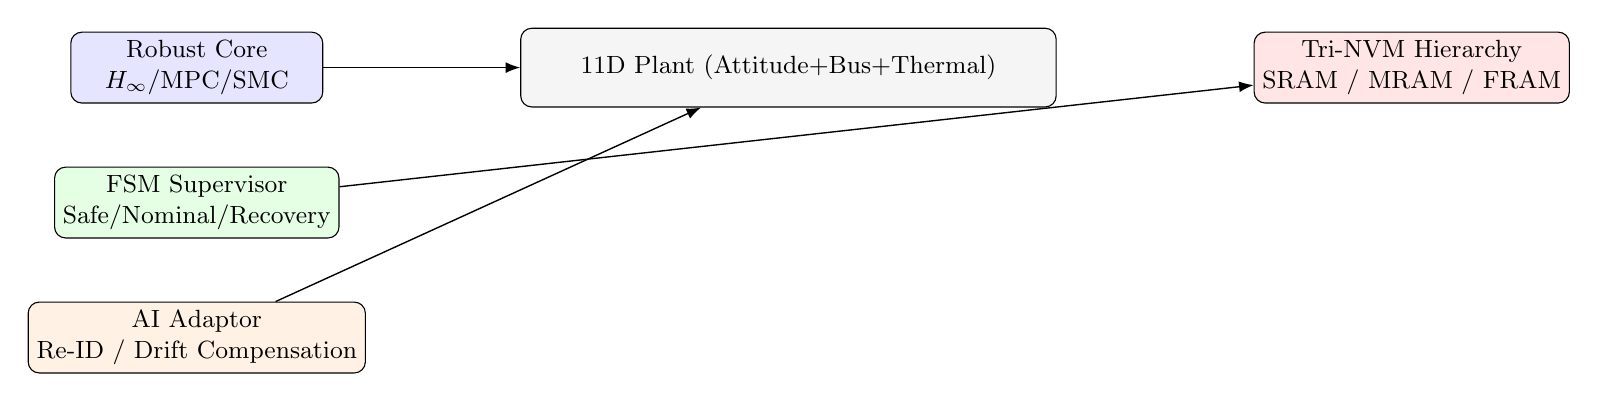
\begin{tikzpicture}[node distance=8mm]
  \node[bigbox, fill=gray!8] (plant) {11D Plant (Attitude+Bus+Thermal)};
  \node[midbox, fill=blue!10, left=25mm of plant] (core) {Robust Core\\$H_\infty$/MPC/SMC};
  \node[midbox, fill=green!10, below=of core] (fsm) {FSM Supervisor\\Safe/Nominal/Recovery};
  \node[midbox, fill=orange!10, below=of fsm] (ai) {AI Adaptor\\Re-ID / Drift Compensation};
  \node[midbox, fill=red!10, right=25mm of plant] (nvm) {Tri-NVM Hierarchy\\SRAM / MRAM / FRAM};

  \draw[line] (core) -- (plant);
  \draw[line] (fsm) -- (nvm);
  \draw[line] (ai) -- (plant);
\end{tikzpicture}
\caption{AITL on Space architecture with three control layers and tri-NVM memory hierarchy.}
\label{fig:arch}
\end{figure*}

% ============================================================
\section{Mathematical Model and $H_\infty$ Design}
We consider an 11D discrete-time state-space plant coupling attitude (6), power bus (2), and thermal nodes (3):
\begin{align}
x_{k+1} &= A x_k + B u_k + E w_k, \\
y_k &= C x_k + D u_k + v_k.
\end{align}
Weights $(W_1, W_2, W_3)$ shape sensitivity, control effort, and complementary sensitivity. EduController outputs plant/weights as JSON. AITL-H synthesizes $K$ with robust stability margins, automatically mapped to fixed-point hardware for FPGA and ASIC targets.

% ---------- Fig.3 Closed-loop ----------
\begin{figure}[t]
\centering
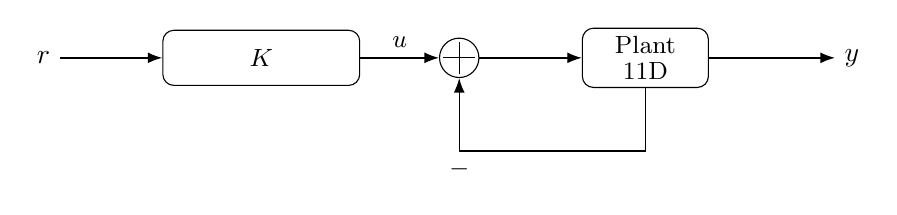
\begin{tikzpicture}[node distance=10mm]
  \node[smallbox] (K) {$K$};
  \node[circle, draw, minimum size=5mm, right=10mm of K] (sum) {};
  \draw (sum) +(-2mm,0) -- +(2mm,0);
  \draw (sum) +(0,-2mm) -- +(0,2mm);
  \node[smallbox, right=13mm of sum, minimum width=16mm] (P) {\shortstack{Plant\\11D}};
  \node[right=16mm of P] (y) {$y$};
  \node[left=13mm of K] (r) {$r$};
  \draw[line] (r) -- (K);
  \draw[line] (K) -- node[above]{\small $u$} (sum);
  \draw[line] (sum) -- (P);
  \draw[line] (P) -- (y);
  \draw[line] ($(P.south)$) |- ++(0,-8mm) -| node[below]{\small $-$} (sum.south);
\end{tikzpicture}
\caption{Closed-loop system for $H_\infty$ mixed-sensitivity synthesis.}
\label{fig:loop}
\end{figure}

% ============================================================
\section{Verification Pipeline}
FPGA HIL injects SEUs and sensor outages. Metrics include safe-mode entry $<\SI{1}{s}$, recovery rate $\ge\SI{99}{\percent}$, and ECC scrubbing efficiency. SystemDK FEM evaluates thermal/radiation stress, validating packaging constraints before ASIC.

% ============================================================
\section{Conclusion}
AITL on Space combines robust control, supervisory safety, AI re-identification, and hardened memory. The proposed end-to-end flow---from JSON specification to ASIC---provides a reproducible methodology for resilient autonomy in long-duration space missions.

% ============================================================
\begin{thebibliography}{99}
\bibitem{doyle}
J.\,C.~Doyle, B.\,A.~Francis, and A.\,R.~Tannenbaum,
\emph{Feedback Control Theory}. Macmillan, 1992.

\bibitem{colinge}
J.-P.~Colinge, \emph{Silicon-on-Insulator Technology: Materials to VLSI}, 3rd~ed. Springer, 2004.

\bibitem{wolf}
W.~Wolf, \emph{FPGA-Based System Design}. Prentice Hall, 2004.

\bibitem{rabaey}
J.~M.~Rabaey, A.~Chandrakasan, and B.~Nikolic,
\emph{Digital Integrated Circuits: A Design Perspective}, 2nd~ed. Prentice Hall, 2003.
\end{thebibliography}

% ---------- Biography ----------
\section*{Author Biography}
Shinichi Samizo received the M.S.\ degree in Electrical and Electronic Engineering from Shinshu University, Japan. He worked at Seiko Epson Corporation as an engineer in semiconductor memory and mixed-signal device development, and contributed to inkjet MEMS actuators and PrecisionCore printhead technology. He is currently an independent semiconductor researcher focusing on process/device education, memory architecture, and AI system integration. Contact: \texttt{shin3t72@gmail.com}.
\end{document}
